% Created 2024-06-10 Mon 14:06
% Intended LaTeX compiler: pdflatex
\documentclass[11pt]{article}
\usepackage[utf8]{inputenc}
\usepackage[T1]{fontenc}
\usepackage{graphicx}
\usepackage{longtable}
\usepackage{wrapfig}
\usepackage{rotating}
\usepackage[normalem]{ulem}
\usepackage{amsmath}
\usepackage{amssymb}
\usepackage{capt-of}
\usepackage{hyperref}
\usepackage{minted}
\author{Jonathan Peel}
\date{\today}
\title{Constellation}
\hypersetup{
 pdfauthor={Jonathan Peel},
 pdftitle={Constellation},
 pdfkeywords={},
 pdfsubject={},
 pdfcreator={Emacs 29.1 (Org mode 9.7)}, 
 pdflang={English}}
\usepackage{biblatex}

\begin{document}

\maketitle
\tableofcontents

\section{Constellation}
\label{sec:orgdcf79fd}

\subsection{Invoice Forms}
\label{sec:org3c4a0c5}

Invoice forms allow table rows to be added inlinde while capturing data.

These instructions assume knowlage on configuring a standard permssions.
\subsubsection{Basic FLL Setup}
\label{sec:org47d37ac}

\begin{enumerate}
\item Musketeer Configuration
\label{sec:org42dc098}

Three tables are required in Muskteer.

\begin{center}
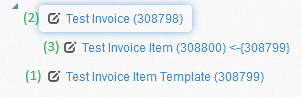
\includegraphics[width=.9\linewidth]{./invoice-basic-setup-fll.png}
\end{center}

\begin{description}
\item[{Item source table (1)}] It is advised that this is a library table.
This holds the deffinitions of items that will be selected on the form.
If the form is for invoices this will hold a list of possible broducs that are being invoiced for.

\item[{Main table (2)}] This is the main table that is used to hold invoices, receiepts, purchase orders, etc.

\item[{Item table (3)}] It is advised that this inherits from the source table, so long that the source table is a library.
This table holds line items of the main record.
These are imported from the source table.
\end{description}
\item Permssion Configuration
\label{sec:org97492df}

Two permissions are required to be created.
\begin{enumerate}
\item The Item permission
\label{sec:org703f1c8}

Needs to reference the item table (3).
\item The Main permssion
\label{sec:org0730f64}

Needs to reference the main table (2).

To add the input table into the form, two things need to be done:

\begin{enumerate}
\item The item permission needs to be added as level 2.

\item A special line needs to be added to the \emph{Form Add} field.
This needs to be in the format ,without spaces, item permission, colon, and the FLL ID of the Item Source table (1), \texttt{item-permission:source-fll}.
\end{enumerate}

\begin{listing}[htbp]
\begin{minted}[frame=leftline,framesep=2mm]{txt}
Title
Description Date Address
invoice-line-items:1234
\end{minted}
\caption{\emph{Form Add} example.}
\end{listing}
\end{enumerate}
\end{enumerate}
\end{document}
